
\documentclass[12pt]{article}

\usepackage{physor2016}

\usepackage{amsmath}
\usepackage{bm}

\usepackage{graphicx}
\usepackage{tikz}
\usepgflibrary{shapes.geometric}

\usepackage{booktabs}

\usepackage{siunitx}
%------------------------------------------------------------------------------

%------------------------------------------------------------------------------
% Define title. Use all CAPITALS.
%------------------------------------------------------------------------------
\title{AN ANGLE-INFORMED HYBRID METHOD FOR DEEP-PENETRATION RADIATION TRANSPORT APPLIED TO CADIS AND FW-CADIS}
%
% ...and authors
%
\author{ 
  \textbf{Madicken Munk and R.~N.~Slaybaugh} \\
  Department of Nuclear Engineering, University of California, Berkeley \\
  3115B Etcheverry Hall, Berkeley, CA 94720, USA\\
  \href{mailto:madicken@berkeley.edu}{madicken@berkeley.edu}\\
  \href{mailto:slaybaugh@berkeley.edu}{slaybaugh@berkeley.edu}\\
  \\
  \textbf{T.~M.~Pandya, Seth R.~Johnson, and T.~M.~Evans}\\
  Radiation Transport Group\\
  Oak Ridge National Laboratory, P.O.\ Box 2008, Oak Ridge, TN 37831, USA\\
  \href{mailto:pandyatm@ornl.gov}{pandyatm@ornl.gov}\\
  \href{mailto:johnsonsr@ornl.gov}{johnsonsr@ornl.gov}\\
  \href{mailto:evanstm@ornl.gov}{evanstm@ornl.gov}
  }
  
%------------------------------------------------------------------------------
\renewcommand{\shortauthor}      % Author's names here
           {M.\ Munk~et~al.}  
\renewcommand{\shorttitle}       % Short title here
           {Angle-Informed CADIS and FW-CADIS}  

%------------------------------------------------------------------------------
% Setup PDF info. This sets several values which are listed as the "properties"
% of the PDF file.
%------------------------------------------------------------------------------
\hypersetup{
  pdftitle=\shorttitle,
  pdfauthor=\shortauthor
}


\begin{document}

%\doublespacing

%\linenumbers

%------------------------------------------------------------------------------
% Make the titlepage and set the pagestyle to fancy throughout
%------------------------------------------------------------------------------
\maketitle

\begin{abstract}
This is our abstract
\end{abstract}

\keywords{Hybrid Methods, CADIS, FW-CADIS, Angular Biasing}

%------------------------------------------------------------------------------
%
%------------------------------------------------------------------------------
\section{INTRODUCTION}
\label{sect::intro}

Efficiently modeling radiation transport in deep penetration shielding problems is essential to the safe operation of many types of nuclear facilities as well as the development of monitoring and detection systems. We would like to be able to perform such calculations with Monte Carlo (MC) methods, but it can be quite challenging to obtain acceptable statistical uncertainties in the computed tallies. Thus, many variance reduction (VR) strategies, some of which we will discuss, have been developed to facilitate accurate calculations in reasonable times. 

An additional challenge, however, is added for problems that exhibit a strong degree of angular anisotropy in particle flux. 
Many existing VR methods do not include angular information in their techniques, and therefore do not work well for these problems.  
Some VR methods do include angular information, but in general these methods have challenges in breadth of applicability or ease of use that make them inadequate as broad tools, or are too costly to use reliably in practice.

With the goal of filling some of these gaps, we have developed a new method that builds on the Consistent Adjoint Driven Importance Sampling (CADIS) and Forward Weighted-CADIS (FW-CADIS) methods~\cite{wagner_forward-weighted_2007} to tackle fixed-source problems that exhibit a high degree of angular anisotropy. 
This method builds on existing software infrastructure in a way that facilitates easy adoption.
CADIS and FW-CADIS, which we will jointly refer to FW/CADIS, use scalar flux estimates from a deterministic calcualtion to create VR parameters for use in MC.
Our new method uses a forward-weighted adjoint scalar flux based on a normalized contributon flux instead of a standard scalar flux.
This new integration scheme includes angular information in order to improve MC performance for problems with anisotropic particle fluxes.

We have implemented this method and tested it on an optically-thick source-detector labyrinth demonstration problem. 
This demonstration problems has characteristics that are particularly challenging for existing methods and provides an opportunity to deeply investigate differences between this new method and CADIS.
As such, we compare an analog calculation, a standard CADIS calculation, and a new angular CADIS calculation
% we need to use a real name here%
, which show that [Talk about the results that we have here]. 

In this paper, we begin with a brief background (Section~\ref{sect::second}) of important concepts relating to variance reduction and existing hybrid methods for deep-penetration radiation transport.
We then provide the context of existing methods in Section~\ref{sec::past}. 
Section~\ref{sect::methodology} describes the mathematical foundation of our proposed method (Section~\ref{subsect::theory}) and the software that we used to implement it (Section~\ref{subsect::implementation}). 
The results and accompanying discussion are described in Section~\ref{sect::results}. Following this, Section~\ref{sect::future} presents our future test plans and details how this plan will map out the application space beyond this single demonstration test. 
We conclude in Section~\ref{sect::conclusion}. 


%------------------------------------------------------------------------------
%
%------------------------------------------------------------------------------
\section{BACKGROUND}
\label{sect::second}

Intro paragraph describing what is covered in background and why\\
(if makes sense for flow/content) quick statement about types of VR and what we'll focus on\\
Write forward and adjoint importance equation and define terms\\
explain Adjoint = Importance; point out this is a concept frequently used in variance reduction \\
expalin Contributon = Response; give any context about use of contributons \\

\section{PAST WORK}
\label{sec::past}
Highlight the CADIS method \\
Highlight the FW-CADIS method \\
Talk about what problems CADIS and FW-CADIS succeed in, then talk about where they fall short. \\
Introduce angle-informed and angle-biased methods. \\
Higlight AVATAR + shortcomings \\
Highlight Turner \& Larsen's method + shortcomings\\
Conclude section with discussion of what is missing from CADIS/FW-CADIS/Angle Methods to motivate new method. \\

%------------------------------------------------------------------------------
%
%------------------------------------------------------------------------------
\section{METHODOLOGY}
\label{sect::methodology}

Introduce section with goal of our method. \\

%------------------------------------------------------------------------------
%
%------------------------------------------------------------------------------
\subsection{Theory}
\label{subsect::theory}

Show our method equation. \\


\begin{equation} 
\label{eq:angularhybrid}
\phi^{+}(\vec{r},E) = \frac{\int \psi(\vec {r} ,E,\hat{\Omega})\psi^+(\vec {r} ,E,\hat{\Omega})d\hat\Omega }{\int\psi(\vec {r} ,E,\hat{\Omega})d\hat\Omega}
\end{equation}


Discuss how this relates to the concept of importance with the adjoint. \\
Discuss how this relates to contributon response. \\
Say physically how this helps us track in problems with strong anisotropy. \\
Highlight how this is different from past methods.

%------------------------------------------------------------------------------
%
%------------------------------------------------------------------------------

\subsection{Implementation}
\label{subsect::implementation}

We implemented this new method through the AutomateD VAriaNce reducTion Generator (ADVANTG)~\cite{wagner_automated_2002, mosher_new_2010} software developed at ORNL. 
ADVANTG automates the generation of the importance map and biased source distribution created using either the CADIS or FW-CADIS methods for use in MCNP5~\cite{brown_mcnp_2002}. 
An input file in MCNP syntax is provided by the user in addition to some instructions for running ADVANTG. 
ADVANTG uses this information to generate input file(s) and exectues the discrete ordinates solver Denovo~\cite{evans_denovo:_2010} in adjoint or forward and adjoint mode, as appropriate.
The deterministic calculations can be performed using multiple cores and/or processors (e.g., on multi-core desktop systems and clusters). 
ADVANTG takes Denovo's output, executes the CADIS or FW-CADIS methods, and the final variance reduction parameters are output in a format that can be used with unmodified versions of MCNP. 
The primary objective of the development of ADVANTG has been to reduce both the user effort and the computational time required to obtain accurate and precise tally estimates
across a broad range of challenging transport application areas.

We chose to use ADVANTG for several key reasons. 
The most important is that the implementation is nearly invisible to the user and therefore their experience of using this method will be nearly identical to using CADIS or FW-CADIS.
That is, the user simply adds an additional instruction asking to use the angle informed method and the interface does not change otherwise.
This facilitates easy adoption.
Further, only one MCNP input file is required to compare the new method to FW/CADIS.
Finally, it was simpler to implement the new method through ADVANTG than starting separately as we could take advantage of so much existing infrastructure in the coupling.

The major modifications required to implement this method were to Denovo. 
The angular flux is typically not stored or written as the desired output is typically the scalar flux.
The new method, however, requires the angular flux to create the scalar flux, and therefore Denovo was modified to store and write the angular flux.
A new function was also added that takes the forward and adjoint fluxes and performs the integration indicated in eqn.~\eqref{eq::angularhybrid}. 
This set of scalar fluxes is then written the way any scalar flux output from Denovo would be.

The benefit the bulk of the implementation being in Denovo is several fold. 
From the standpoint of ADVANTG, there are very few differences between the new method and FW/CADIS and therefore implementation is straightforward.
Further, anyone who finds a use for a scalar flux created as in eqn.~\eqref{eq::angularhybrid} will now be able  access it.
Finally, it might be useful to have access to the full angular flux. 
Examining the angular flux for a problem could have research or pedagogical implications, and some other variance reduction method that uses the angular flux explicitly could be more easily developed in the future.

%------------------------------------------------------------------------------
%
%------------------------------------------------------------------------------
\section{RESULTS AND DISCUSSION} 
\label{sect::results}

Show test problem geometry

Image I: problem geometry \\

\begin{figure}
  \begin{center}
    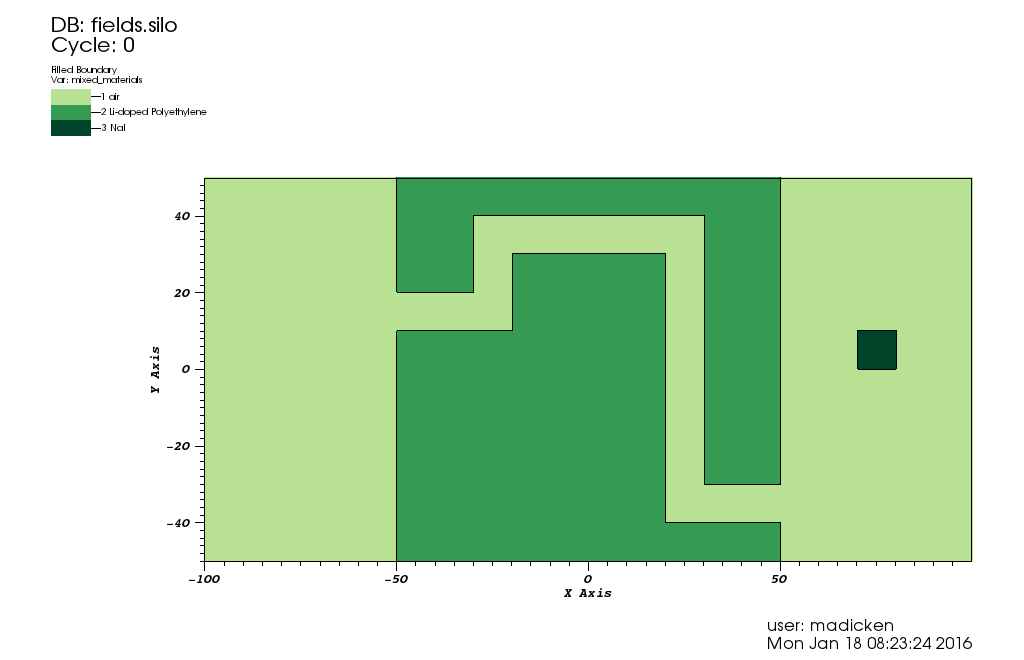
\includegraphics[width=0.8\textwidth]{./images/geometry0000.png}
    \caption[]{\label{fig::geometry}Labyrinth I geometry: A multi-legged air duct through polyethylene with a point source at (-75, 0, 0) and a NaI detector behind the polyethylene shield.}
  \end{center}
\end{figure}

Image II: tally results for NaI response \\
Image III: tally uncertainties for NaI response \\

Forward flux for problem \\
\begin{figure}
  \begin{center}
    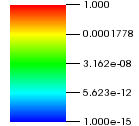
\includegraphics[width=0.10\textwidth]{./images/scale.png}
    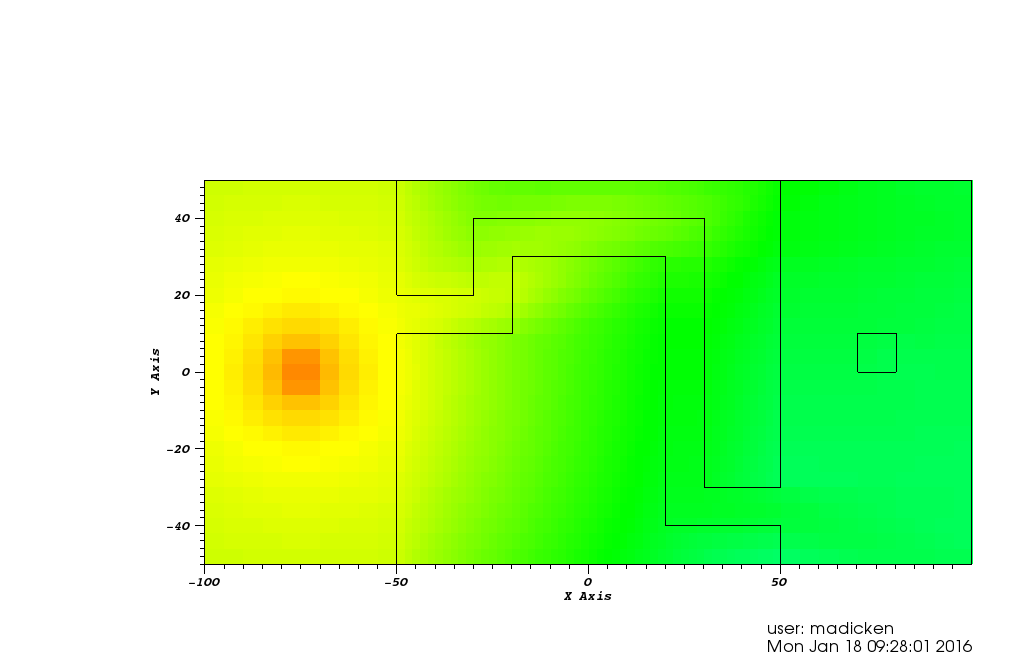
\includegraphics[width=0.80\textwidth]{./images/forward_flux.png}
    \caption[]{\label{fig::fwdflux}Forward flux generated by Denovo}
  \end{center}
\end{figure}

Adjoint flux map for problem \\
\begin{figure}
  \begin{center}
    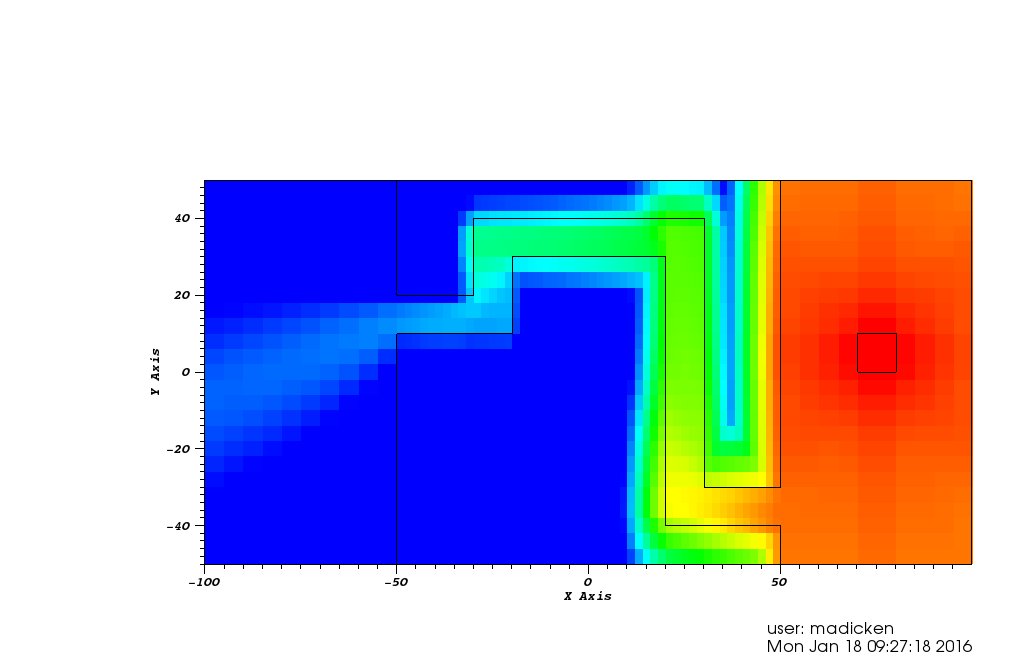
\includegraphics[width=0.80\textwidth]{./images/adjoint_flux.png}
    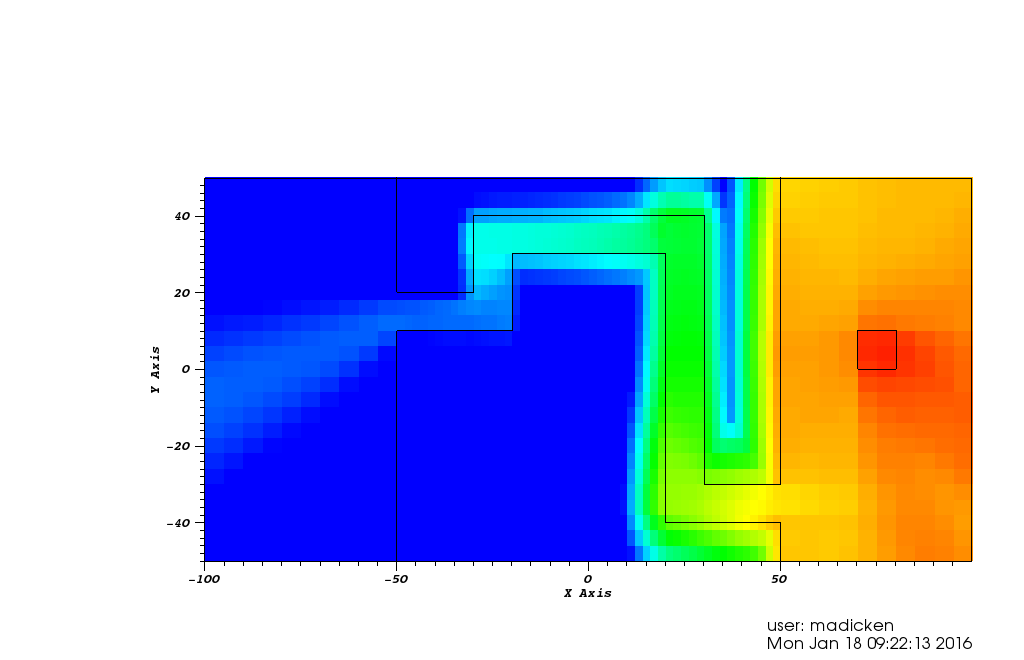
\includegraphics[width=0.80\textwidth]{./images/our_flux.png}
    \caption[]{\label{fig::otherflux}Adjoint flux generated by Denovo and Adjusted adjoint flux with forward-weighting.}
  \end{center}
\end{figure}

Forward-weighted adjoint flux for problem \\
Discuss differences and meaning of differences of results and parameter maps \\
Discuss implications of these differences for solving other problems more generally \\


 \begin{table}
  \centering
  \caption{\label{tab:FOMLabI}FOMs for Labyrinth I}
  \begin{tabular}{l|c}
    \toprule
    -- & FOM\\
    \hline
    Analog           & 12 \\ 
    CADIS            & 340 \\
    Angular CADIS    & --- \\  
	\bottomrule
  \end{tabular}
\end{table}

%------------------------------------------------------------------------------
%
%------------------------------------------------------------------------------
\section{FUTURE WORK} 
\label{sect::future}

Show the future test phase space we plan to cover. 

The testing phase of this project aims to (1) characterize the method's performance in a variety of problems that have anisotropies, and (2) compare how well the method performs compared to traditional CADIS and FW-CADIS.
The goal of the former is to determine in which situations the method performs best, and the latter aims to quantify the extent to which the method is successful. 
Table \ref{tab:testprobs} summarizes a selection of test problems that have shown difficulty for CADIS and FW-CADIS as well as additional problems that the authors expect to have strong angular anisotropy. 
In particular, problems where the direction of the particles is relevant to the importance of a cell will be relevant to characterizing the proposed method. 
Each of these problems has some angular anisotropy, but have different physical means by which this anisotropy is created. 
This selection of test problems should help to inform what types of larger systems and problems the method will be useful to optimize. 


 \begin{table}
  \centering
  \caption{Proposed Test Problem Coverage}
  \begin{tabular}{l|cccc}
    \toprule
    Problem Name & \multicolumn{4}{c}{Problem Coverage} \\
    \hline
    -- & Streaming Paths & Highly Scattering & Highly Heterogenous & Beam Problem \\
    \hline
    Streaming Channel   & X & & & X \\ 
    Metal Plate         & X & X & X &  \\
    Labyrinth Variants  & X & X & X &  \\ 
    Spherical Boat      & X & & X & X \\  
    Kobayashi Benchmark & X & X &  &  \\   
	\bottomrule
  \end{tabular}
  \label{tab:testprobs}
\end{table}



%------------------------------------------------------------------------------
%
%------------------------------------------------------------------------------
\section{CONCLUSION} 
\label{sect::conclusion}

Recap what we told them (what problem we're trying to solve; about this method; how it's different than past methods)\\
Recap problem we solved and results\\
Strong punchline paragraph about potential impact based on theory and these results.

%------------------------------------------------------------------------------
%
%------------------------------------------------------------------------------
\section*{ACKNOWLEDGMENTS}

This material is based on work supported by the Department of Energy under award number DE-NE0008286. This report was prepared as an account of work sponsored by an agency of the United States Government. Neither the United States Government nor any agency thereof, nor any of their employees, makes any warranty, express or implied, or assumes any legal liability or responsibility for the accuracy, completeness, or usefulness of any information, apparatus, product, or process disclosed, or represents that its use would not infringe privately owned rights. Reference herein to any specific commercial product, process, or service by trade name, trademark, manufacturer, or otherwise does not necessarily constitute or imply its endorsement, recommendation, or favoring by the United States Government or any agency thereof. The views and opinions of the authors expressed herein do not necessarily state or reflect those of the United States Government or any agency thereof.

\bibliographystyle{physor2016}
\bibliography{physor2016}

\appendix

\makeatletter
\def\@seccntformat#1{APPENDIX \csname the#1\endcsname.~}
\makeatother

%------------------------------------------------------------------------------
% If you need to make one (or more) appendix (appendices), place them here as
% sections
%------------------------------------------------------------------------------
\section{HOW TO MAKE APPENDICES}
\label{app::a}

This is a placeholder for my first appendix

\section{OTHER APPENDIX STUFF}
\label{app::b}

This is a placeholder for my second appendix

\end{document}

